% Définition du répertoire contenant les images
\graphicspath{{IMAGE/}}

% FRAME Intro
\begin{frame}


\includegraphics[width=12cm]{Logos.pdf}

\vfill

\begin{center}

\vspace*{1.5cm}

\LARGE
\textbf{Density}

\vspace*{1.5cm}
 DELHI GIS-R School


\large
9-12\up{th} April 2019

\vspace*{1.5cm}


\textbf{Hadrien Commenges \& Paul Chapron}

{\small

\vspace*{0.1cm}

\url{hadrien.commenges@univ-paris1.fr}

\url{paul.chapron@ign.fr}
}

\end{center}

\end{frame}

% FRAME
\begin{frame}{Use case}

\begin{block}{Density}
Density is a \textbf{spatial variable} depicting the \textbf{spatial variation} of some observations (concentration and dispersion) in 1, 2 or $n$ dimensions. 
\end{block}

\begin{itemize}
\item Mass / Volume ratio (volumetric mass), mass per volume unit, sometimes ratio between an object volumetric mass and a reference volumetric mass. 
\item Ratio between a \textbf{count}  and its \textbf{extent}: a variable's density (1D), population density (2D, so \textbf{spatial extent}), etc.
\end{itemize}

~

\textbf{What kind of geographical information is concerned ?}

$\rightarrow$ \textit{TYPE 1 - Geographical Objects}

$\rightarrow$ \textit{TYPE 2 - Occurrences}

\end{frame}


% FRAME
\begin{frame}{Goals}

\textbf{Main uses:}

\begin{enumerate}
  \item Describe a point pattern 
  \item Estimate the probability of an event to occur at a given point
  \item Estimate the probability that a spatial distribution of events is random.
\end{enumerate}

\end{frame}


% FRAME
\begin{frame}{Spatial distribution parameters}

\textbf{Centrality} and \textbf{dispersion} can be computed in a 1, 2 2 or $n$ dimensions space. 

~

Current analysis of these parameters:

\begin{itemize}
\item Description of a distribution: mean and standard deviation
\item Evolution of these parameters over time
\item Parameters weight
\end{itemize}

\end{frame}


% FRAME
\begin{frame}{Spatial distribution parameters}

2-Dimensions \textbf{mean}  : \textbf{barycenter} (or \textbf{balancing point } ).

$$
x_g = \frac{\sum_{i=1}^n w_i x_i}{\sum_{i=1}^n w_i} ~~~~~~~~~~~~~~~ y_g = \frac{\sum_{i=1}^n w_i y_i}{\sum_{i=1}^n w_i}
$$

~

~

$\rightarrow$ weights $w_i$ might be constant or varying, depicting localized stocks variations.

\end{frame}



% FRAME
\begin{frame}{Spatial distribution parameters}

2-Dimensions \textbf{variance} $\approx$ \textbf{inertia}.

\begin{figure}
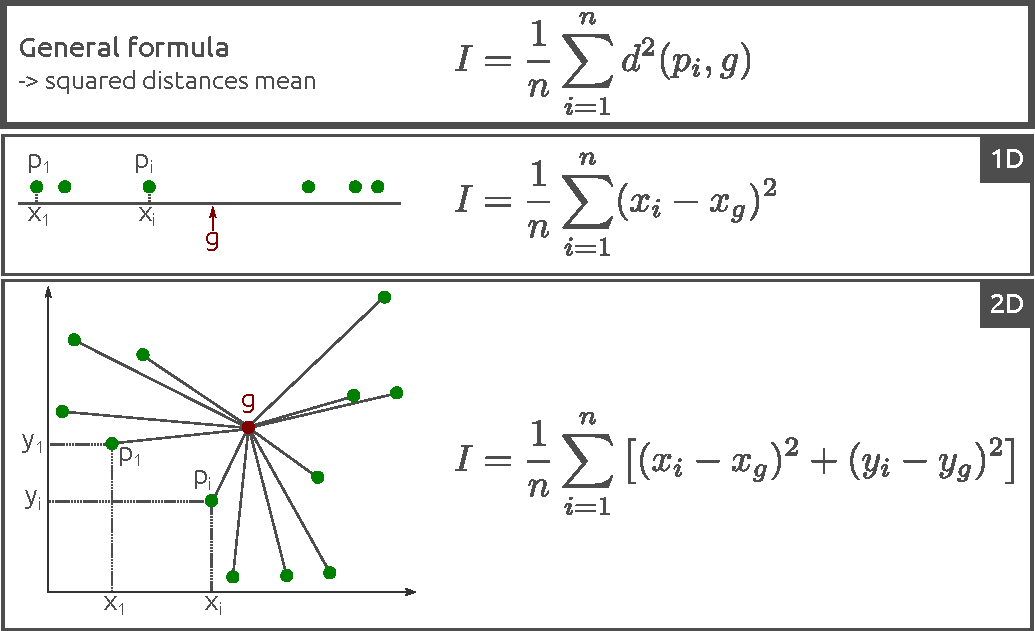
\includegraphics[width=11cm]{Inertie_EN.pdf}
\end{figure}


\end{frame}

% FRAME
\begin{frame}{Spatial distribution parameters}

\begin{figure}
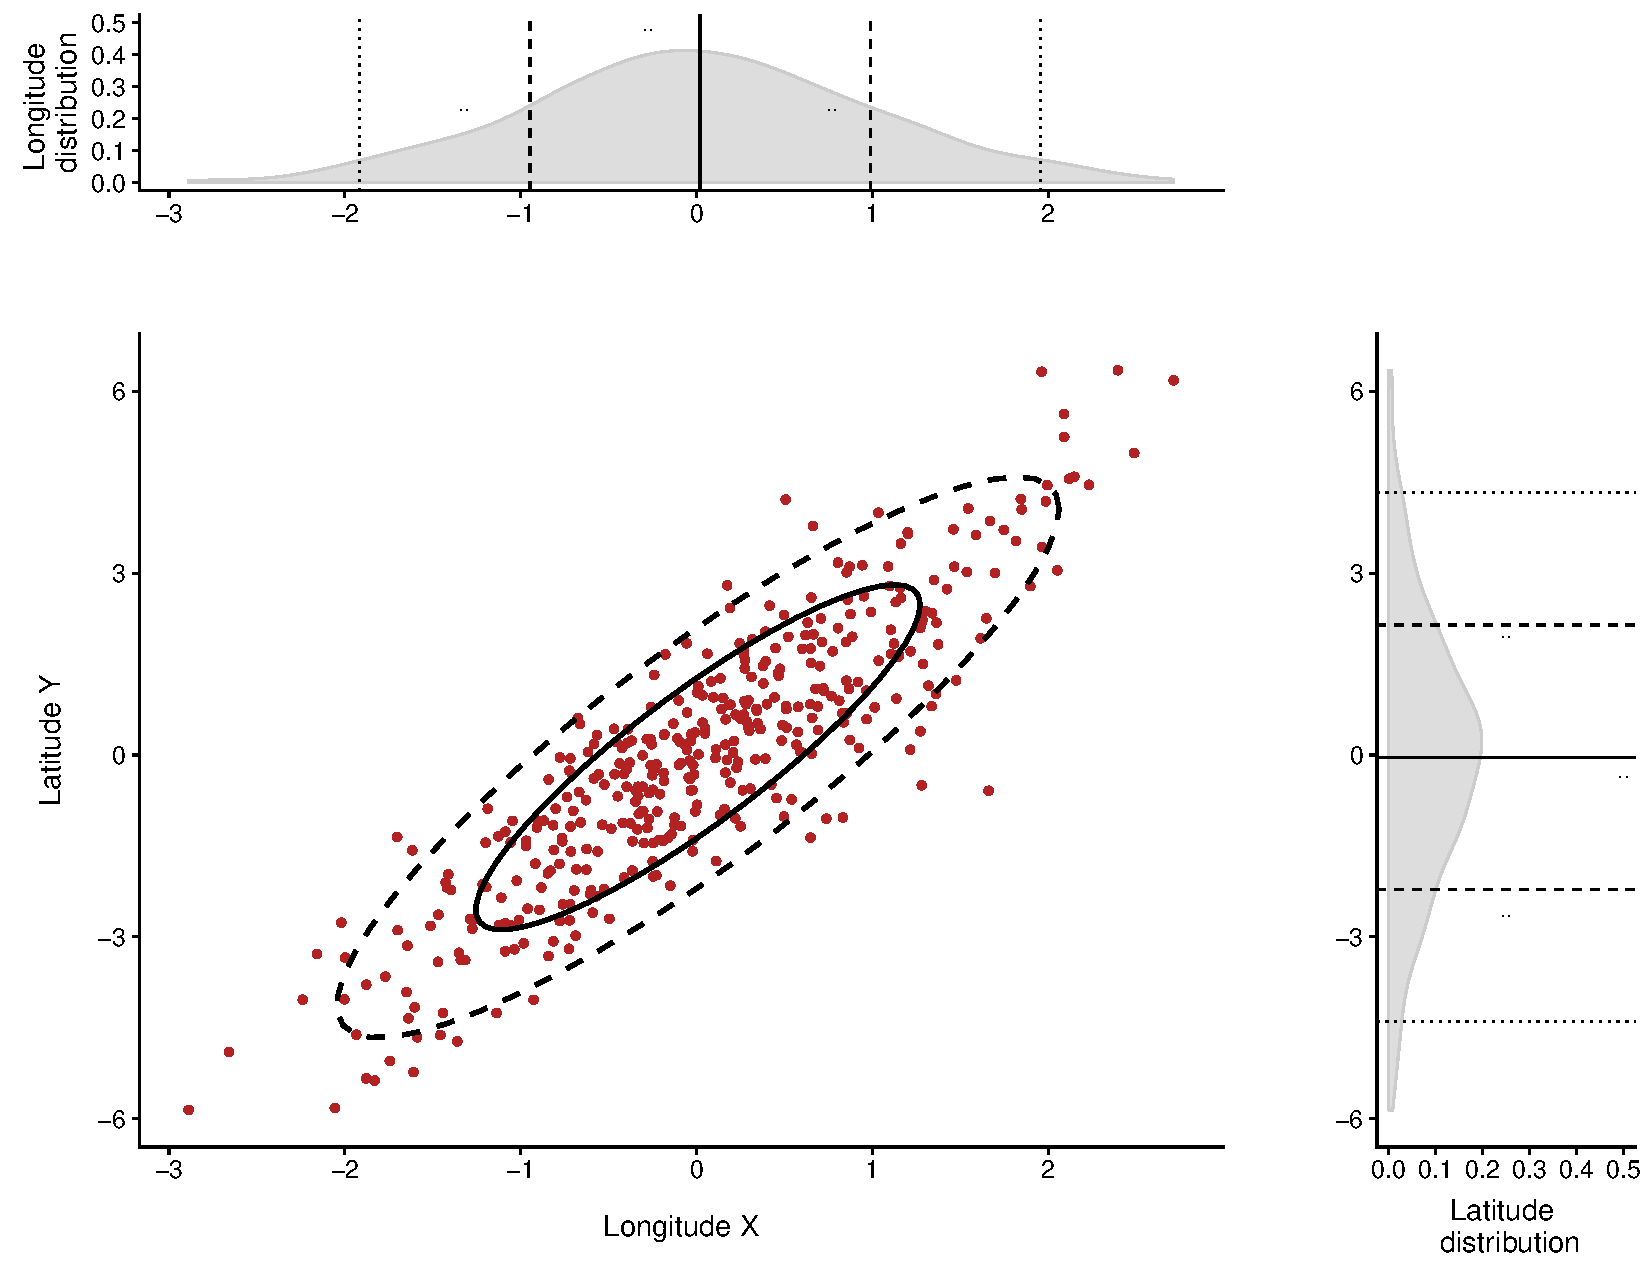
\includegraphics[width=9cm]{Ellipsis_dev_EN.pdf}
\end{figure}

\end{frame}


% FRAME
\begin{frame}{Spatial distribution parameters}

\begin{figure}
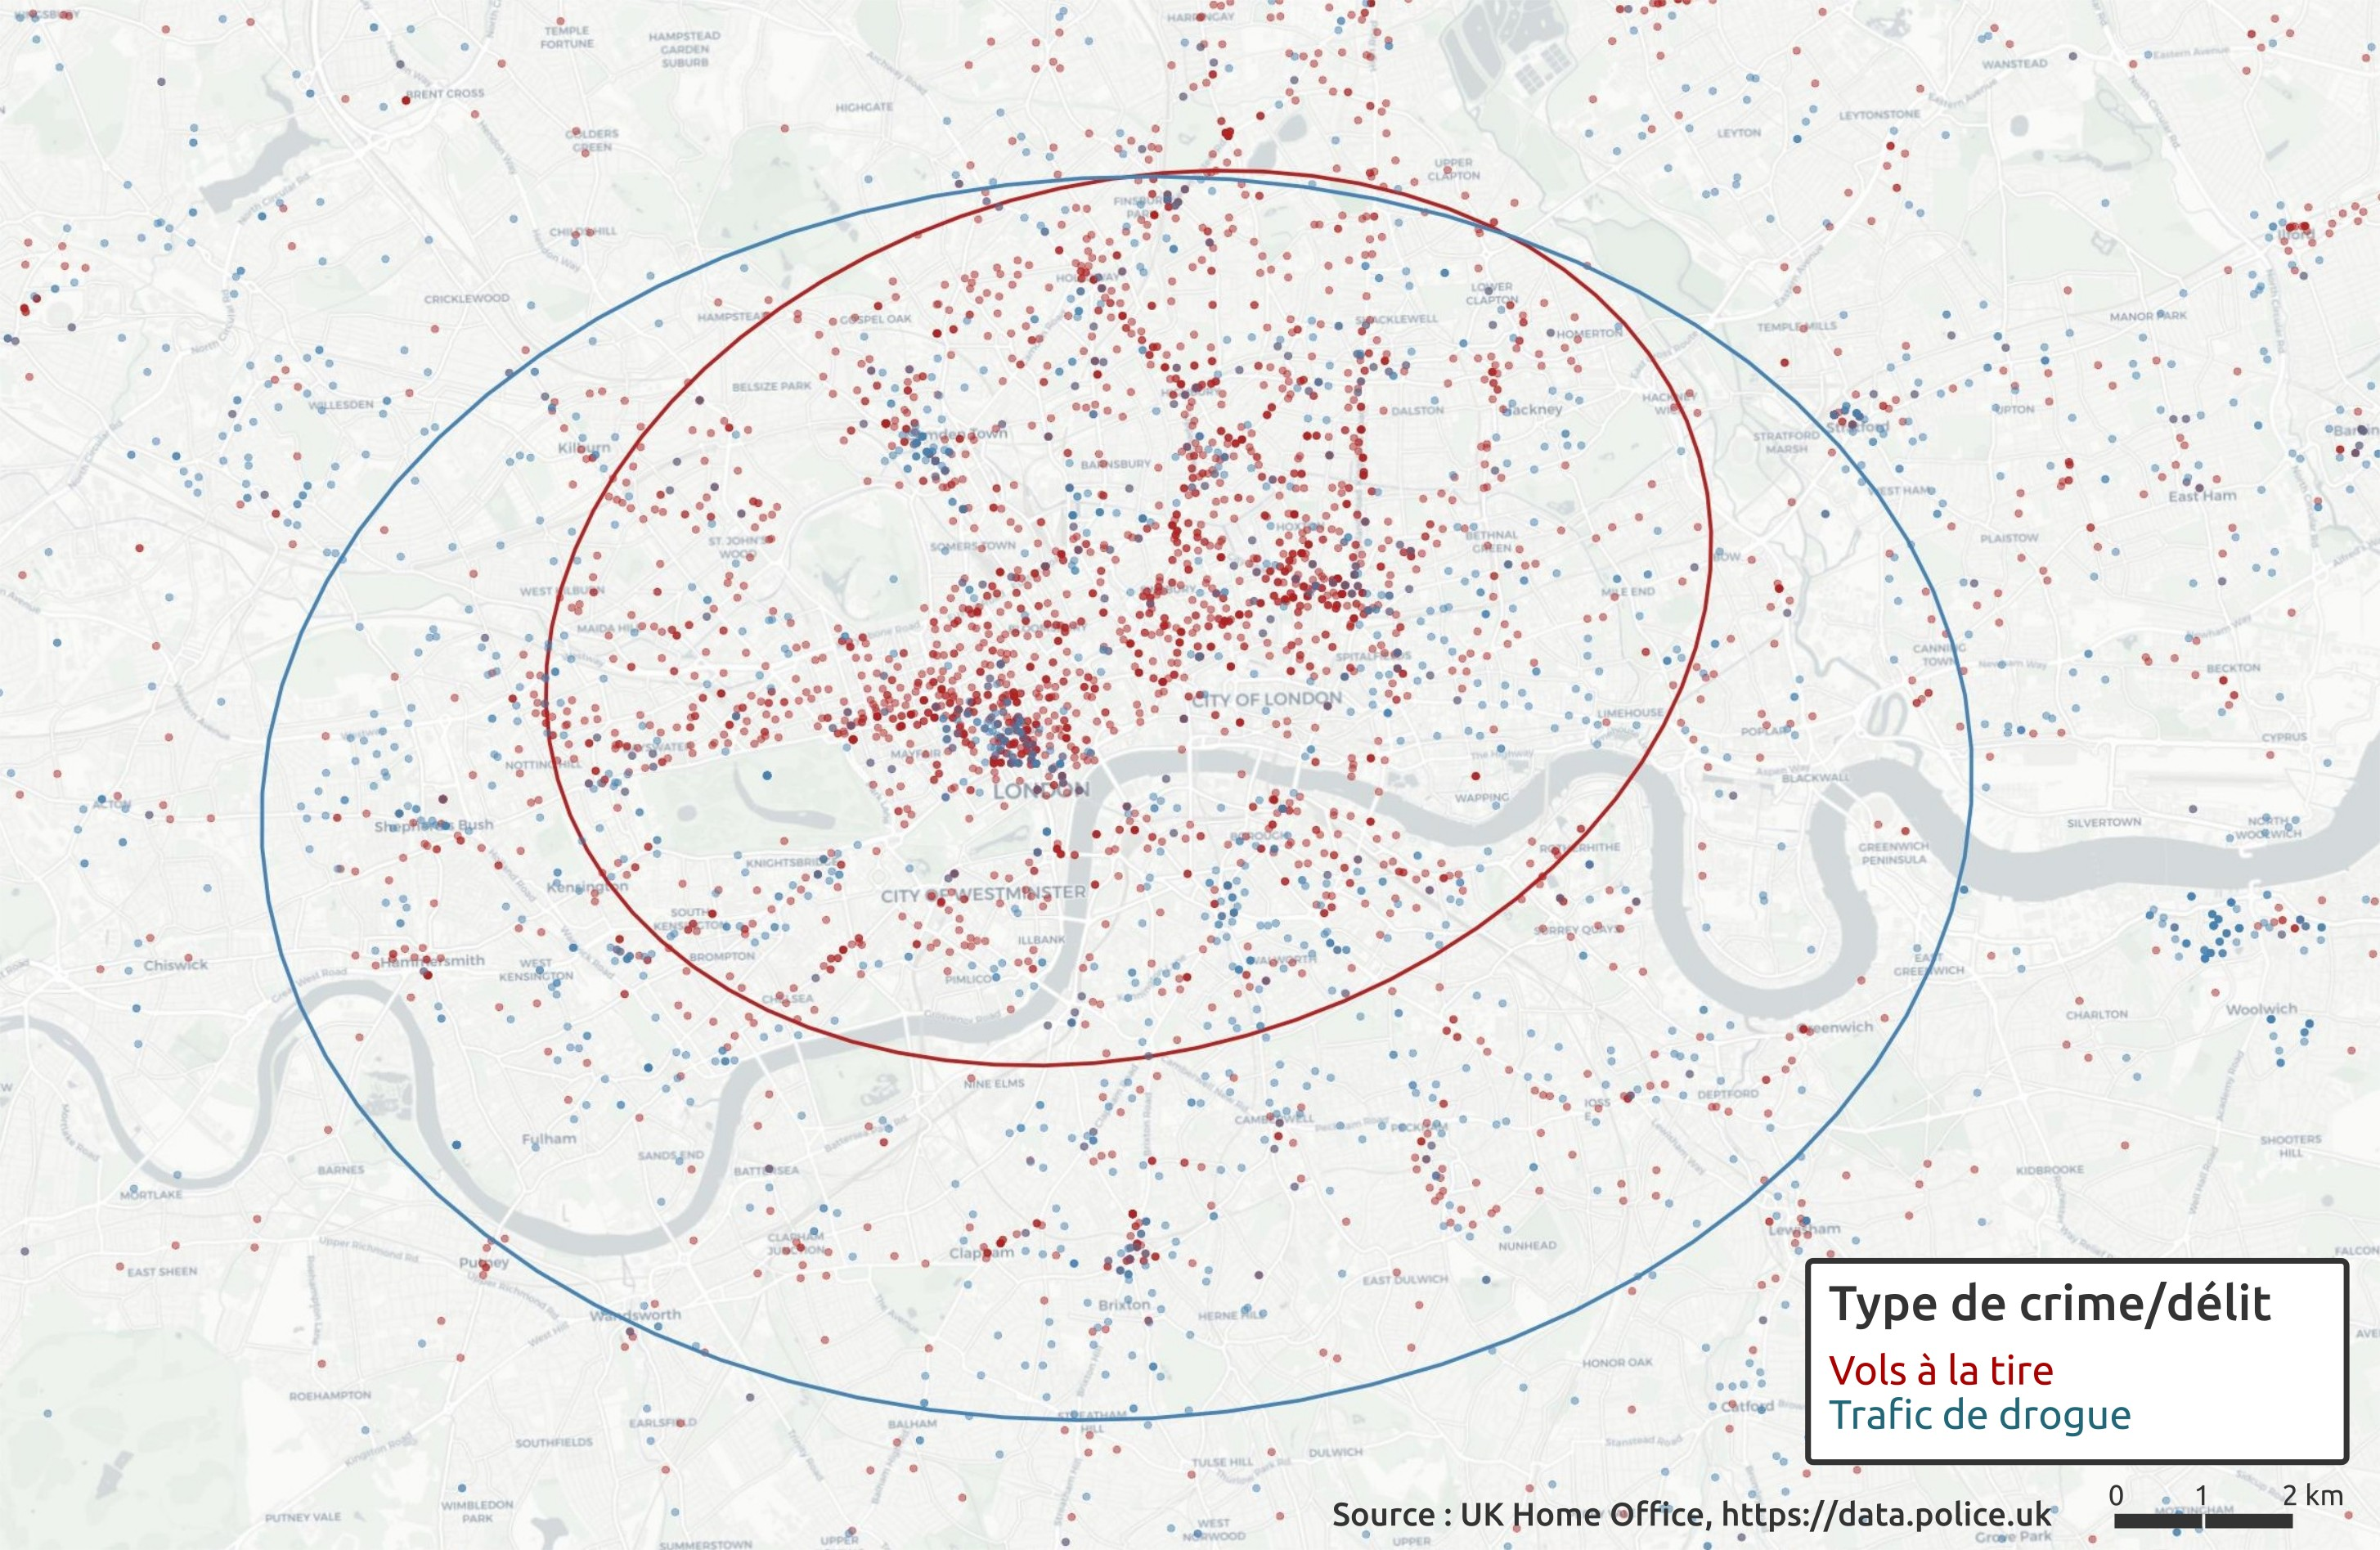
\includegraphics[width=12cm]{Crimes.jpg}
\end{figure}

\end{frame}



% FRAME
\begin{frame}{Spatial distribution parameters}

\begin{figure}
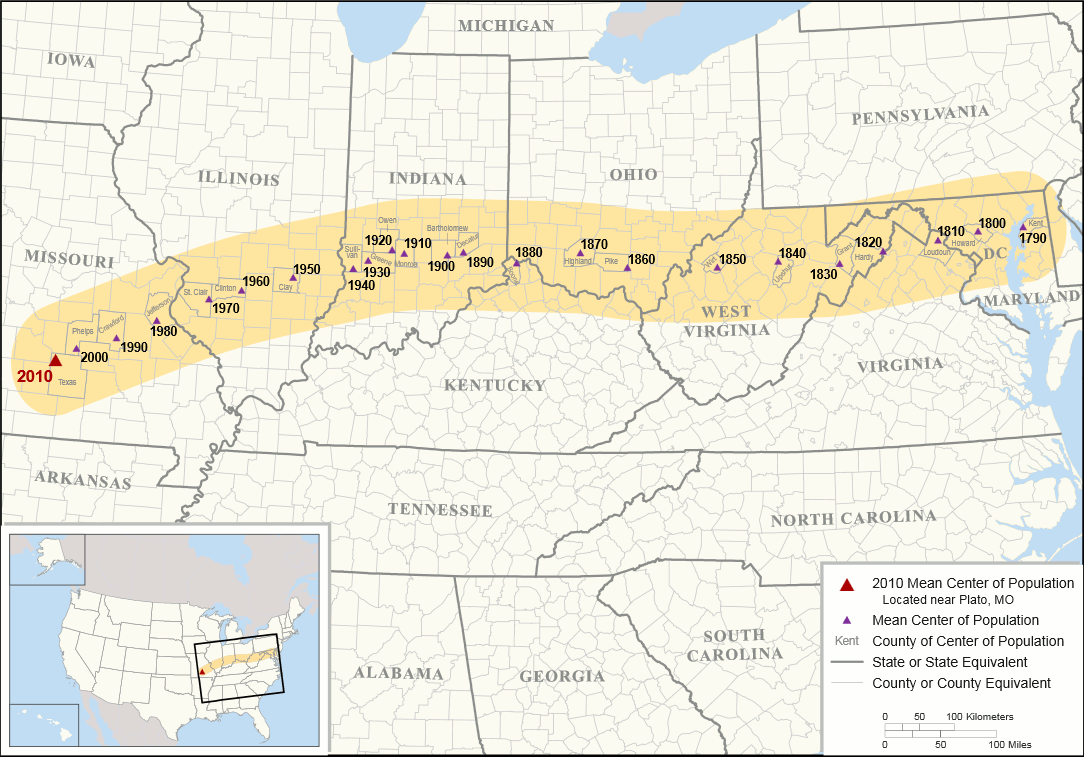
\includegraphics[width=10cm]{Centerpop.png}
\end{figure}

\footnotesize
Source: US Census, \url{https://www.census.gov/geo/reference/centersofpop.html}
\normalsize

\end{frame}


% FRAME
\begin{frame}{1D distribution graph (discrete)}

\textbf{Histogram}

~ 

\begin{figure}
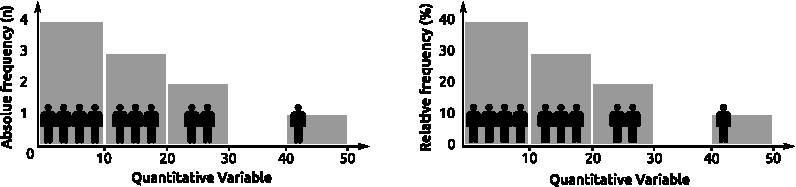
\includegraphics[width=12cm]{Histogramme_EN.pdf}
\end{figure}

$\rightarrow$ histogram estimated density is \textbf{discrete} by construction.

\end{frame}



% FRAME
\begin{frame}{Distribution graph (Parzen)}

\textbf{Histogram generalization: Parzen window}

~ 

\begin{figure}
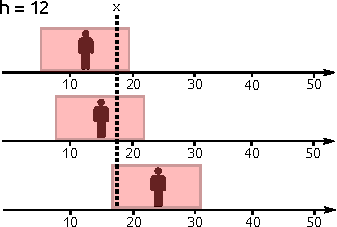
\includegraphics[width=6cm]{HistogrammeParzen.pdf}
\end{figure}

$$ D(x) = \frac{1}{3 \times 12} (1 + 1 + 1) = \frac{1}{12}$$

\end{frame}


% FRAME
\begin{frame}{Distribution graph (continuous)}

\textbf{Parzen Generalization: Gaussian Kernel}

\begin{figure}
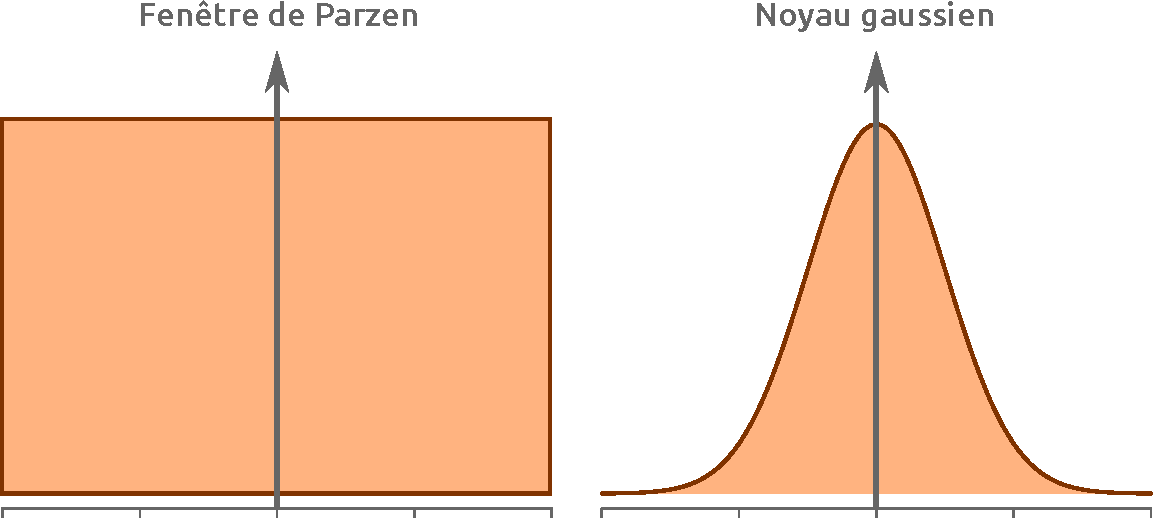
\includegraphics[width=10cm]{Gauss.pdf}
\end{figure}

\end{frame}





\begin{frame}{1D distribution graph (continuous)}

\textbf{Kernel Density Estimate}

General idea: density for a value $x$ is estimated by the proportion of observation \textit{near $x$}  

«Near» is defined by a certain window described by a \textbf{kernel function} (usually gaussian).

Contribution of each observation within the window is given by kernel function value taken for each $x$. $implies$ smoothing


\begin{figure}
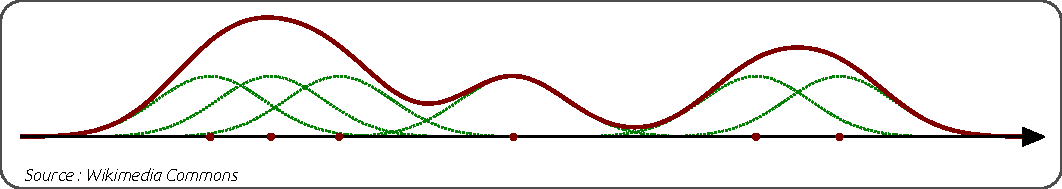
\includegraphics[width=12cm]{KDE.pdf}
\end{figure}

«Close observations contribute strongly, far ones contribute slightly »

~

\textit{Kernel Density Estimator}) may be applied in 1 to $n$ dimensions. 
For spatial analysis, we use the \textbf{2D} version.

\end{frame}


% FRAME
\begin{frame}{Distribution mapping}

Density obtained by (KDE) in \textbf{2 Dimensions}.

\begin{figure}
  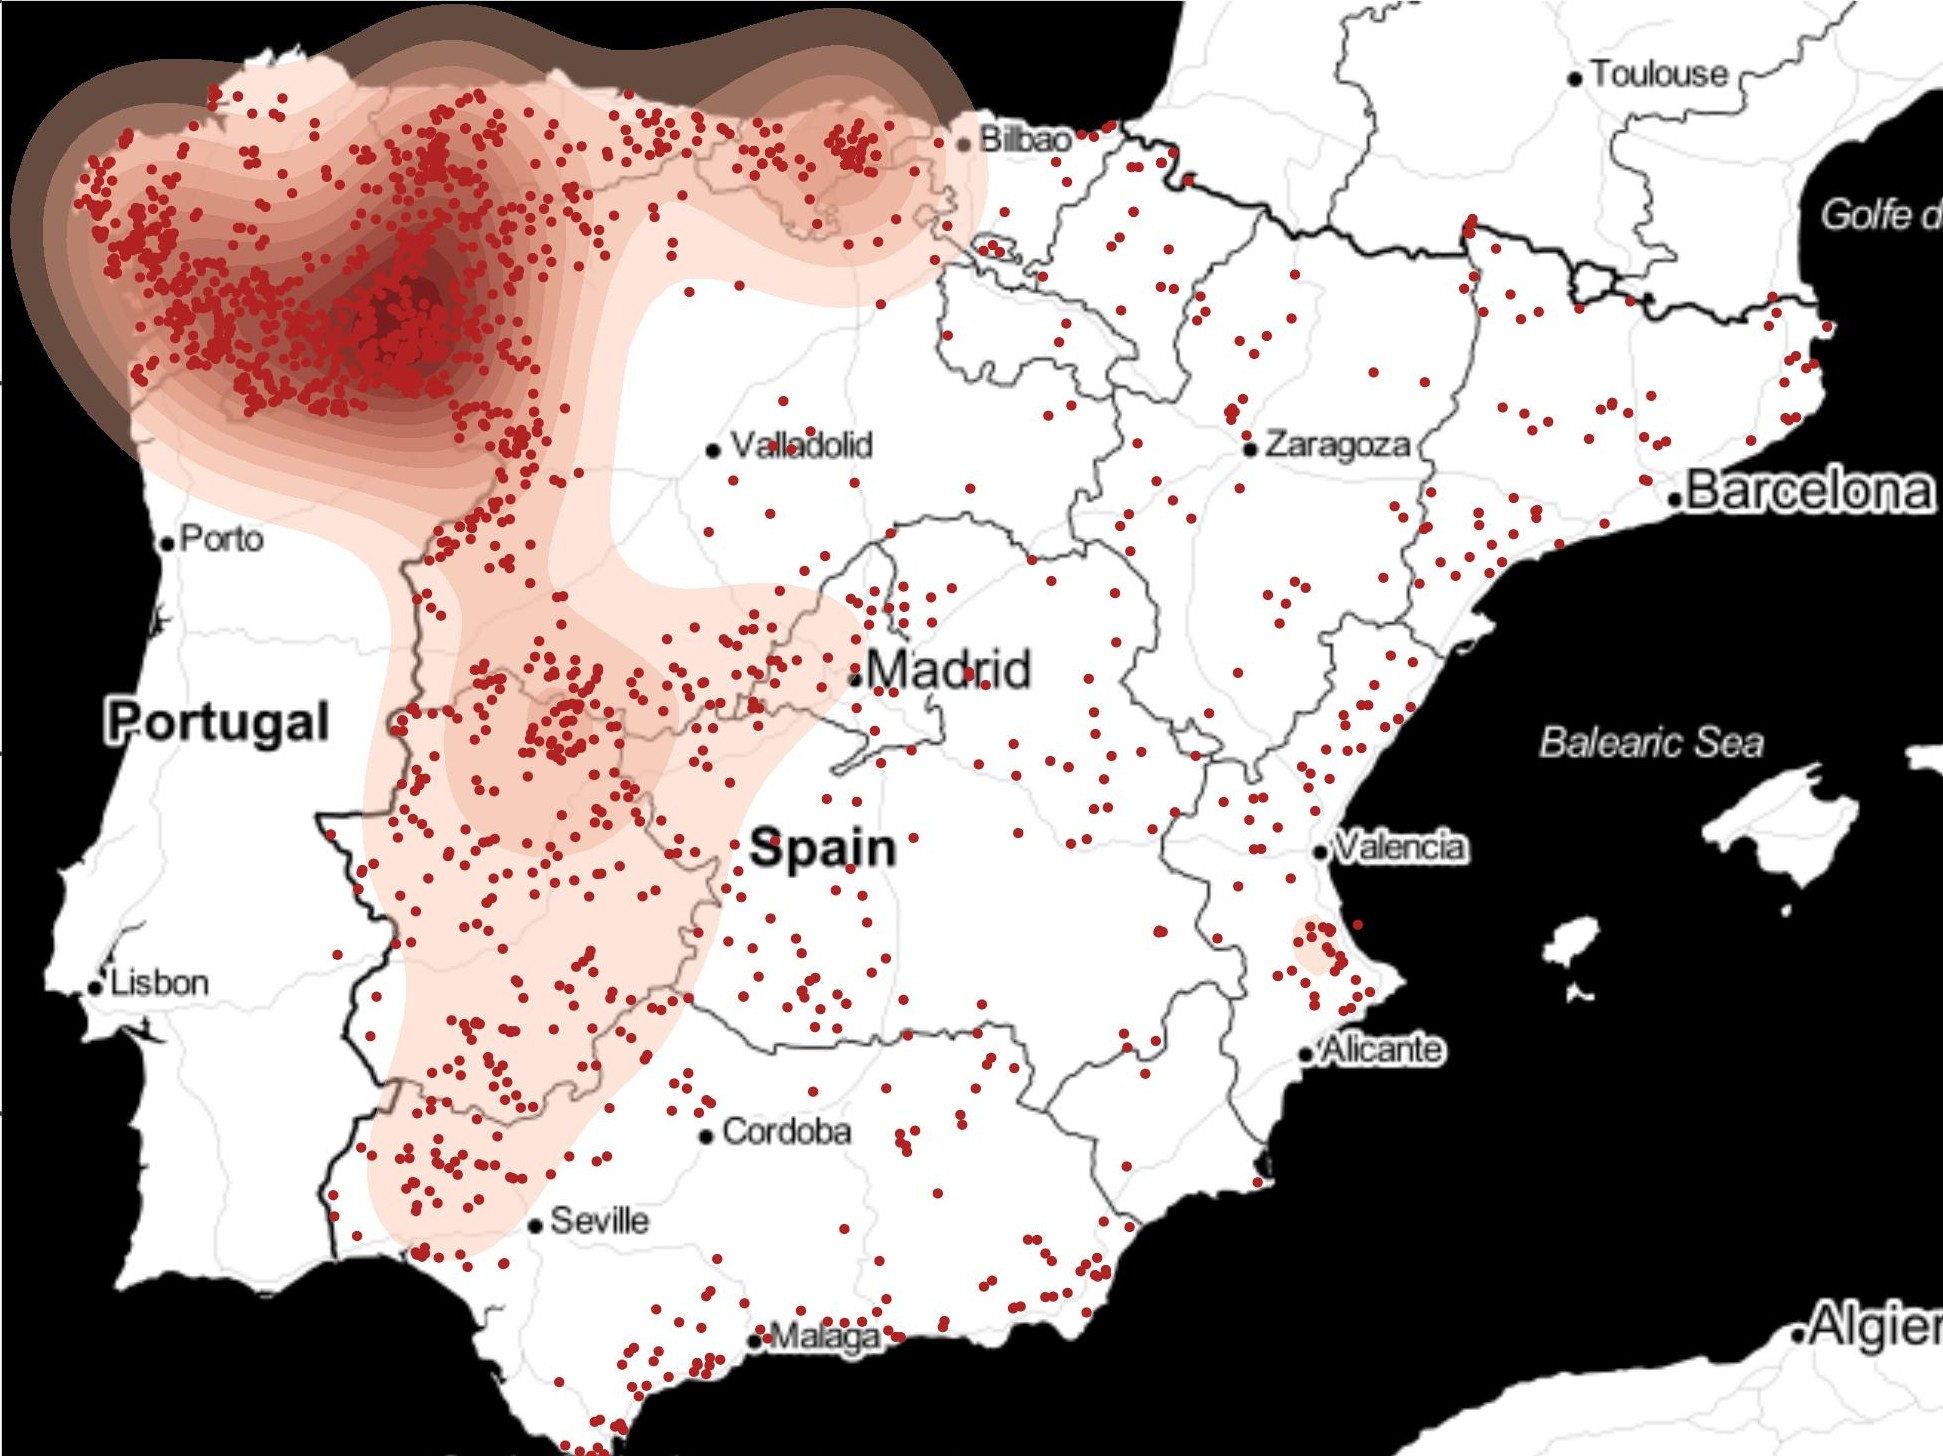
\includegraphics[width=8cm]{Incendies.jpg}
\end{figure}

\end{frame}


% FRAME
\begin{frame}{Distribution testing}

\textbf{May this distribution have been generated by a stochastic process ?}

\begin{figure}
  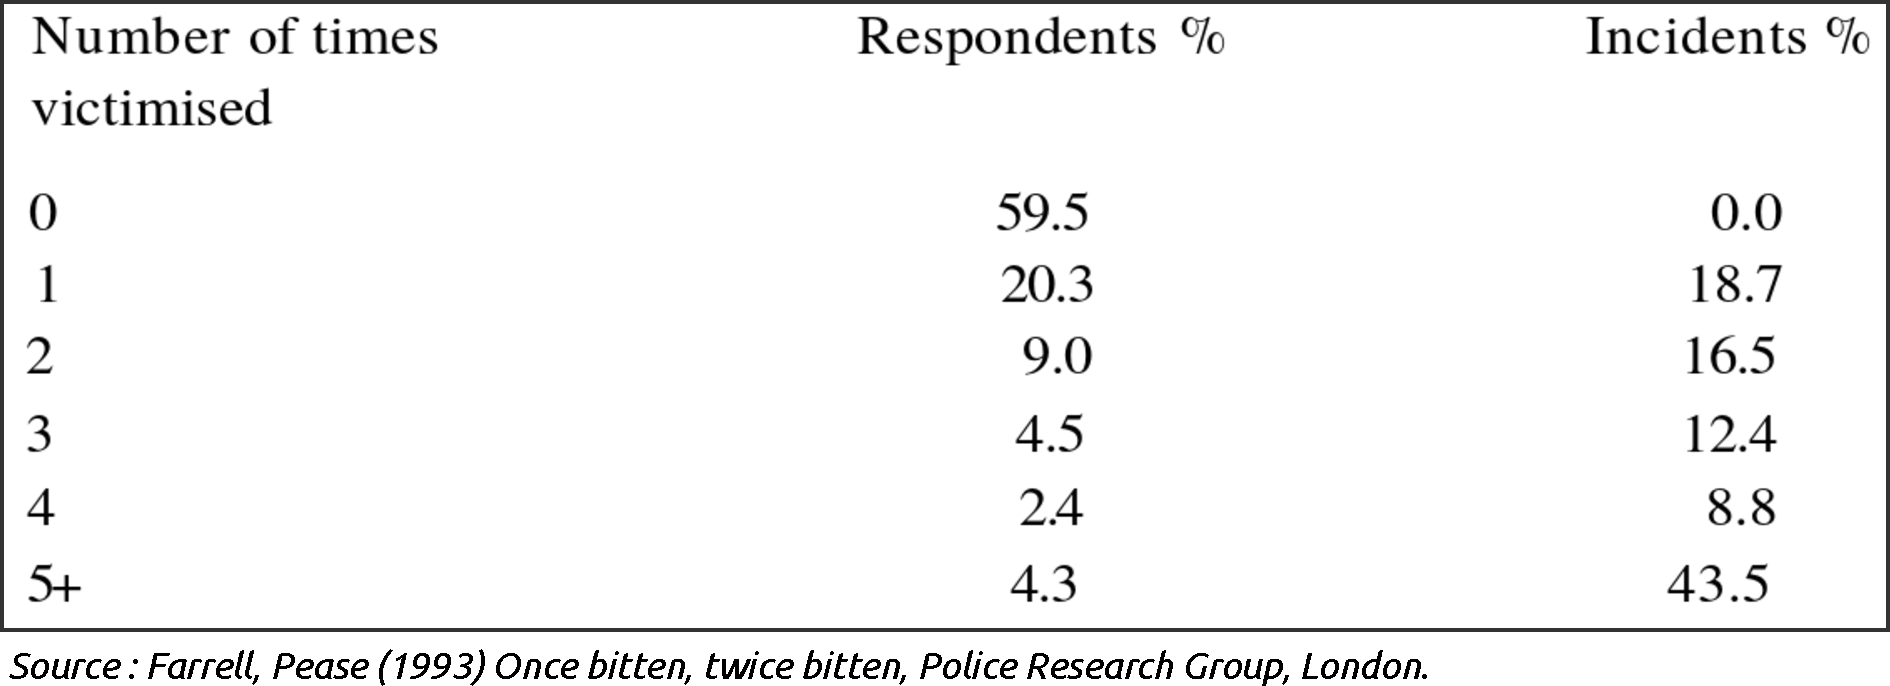
\includegraphics[width=11cm]{CrimeConcentration.pdf}
\end{figure}

\end{frame}


% FRAME
\begin{frame}{Distribution testing}
\textbf{May this distribution have been generated by a stochastic process ?}

\begin{figure}
  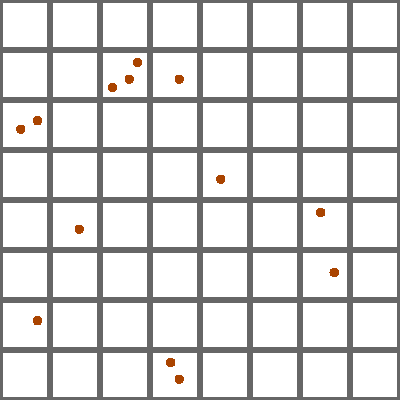
\includegraphics[width=6.5cm]{ExPoisson.pdf}
\end{figure}

\end{frame}


% FRAME
\begin{frame}{Distribution testing}

\textbf{May this distribution have been generated by a stochastic process ?}

\begin{figure}
  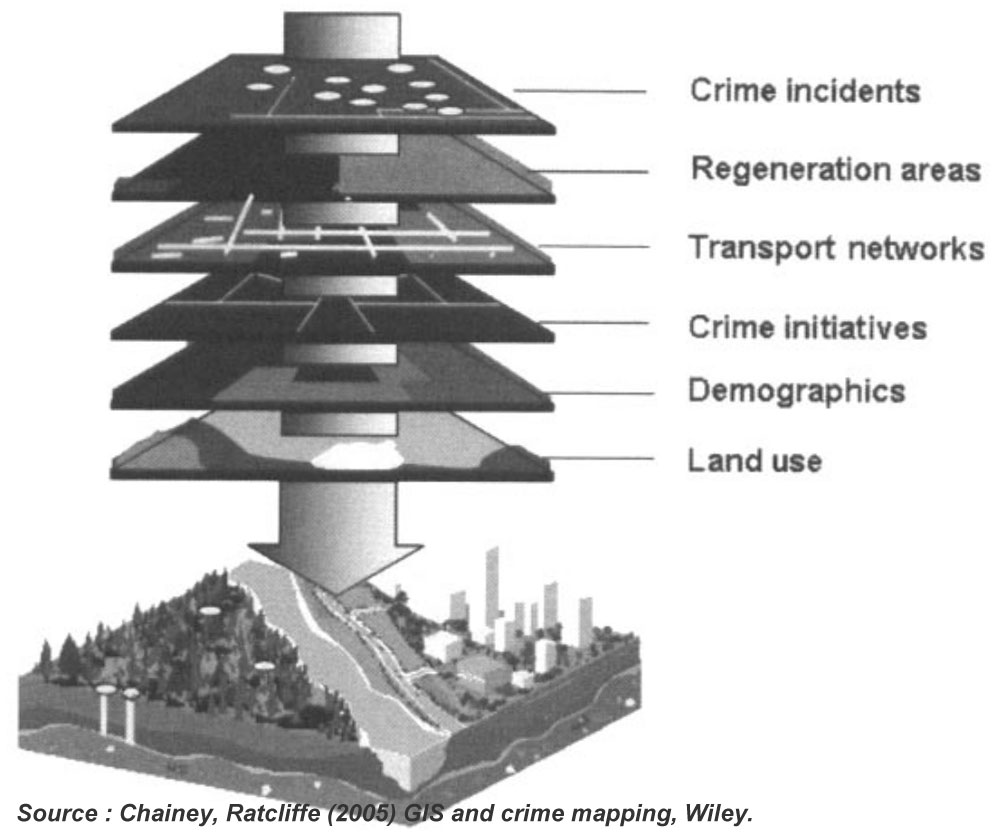
\includegraphics[width=7cm]{Chainey.jpg}
\end{figure}

\end{frame}


% FRAME
\begin{frame}{Poisson distribution}

Poisson's distribution $\lambda$ parameter is both the \textbf{mean} and the \textbf{variance} of the distribution.

\begin{equation}
\nonumber
P(X = k) = \frac{\lambda^k e^{-\lambda}}{k!}
\end{equation}


\begin{figure}
  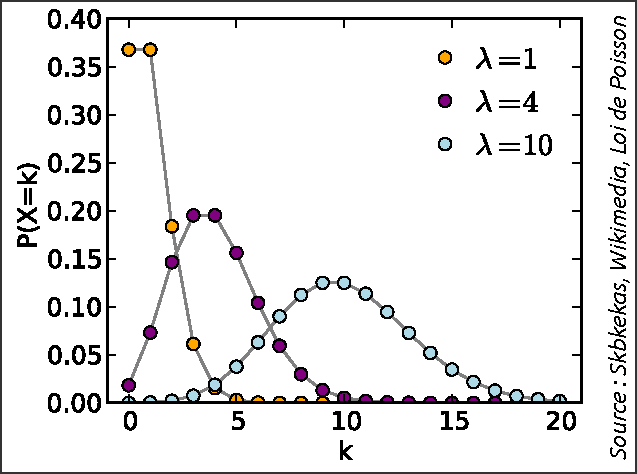
\includegraphics[width=7cm]{Poisson.pdf}
\end{figure}

\end{frame}



% FRAME
\begin{frame}{Poisson spatial distribution}

A \textbf{Poisson spatial process} is a \textbf{spatial stochastic process}, sometimes labelled as :

\begin{itemize}
  \item \textit{spatial Poisson process}
  \item \textit{homogeneous Poisson process}
  \item \textit{complete spatial randomness} (CSR)
\end{itemize}

Given a partitioned space $Z$, the probability of a given number of occurences in a zone $z$ is modeled by a Poisson distribution whose mean is  $\lambda \times area(z)$.

\end{frame}


% FRAME
\begin{frame}{Dispersion index}

\textbf{VMR} \textit{Variance-to-Mean Ratio} $=\frac{\mu}{\sigma^2}$

\begin{itemize}
\item Construct a regular grid 
\item Count occurrences
\item Compute variance,  mean and VMR
\end{itemize}

~

\textbf{VMR intrepretation}

\begin{itemize}
  \item VMR = 0 : not dispersed 
  \item VMR = 1 : may have been obtained by a Poisson process
  \item VMR < 1 : uniform / periodic
  \item VMR > 1 : concentrated / clusters
\end{itemize}

\end{frame}


% FRAME
\begin{frame}{Dispersion index}

\begin{figure}
  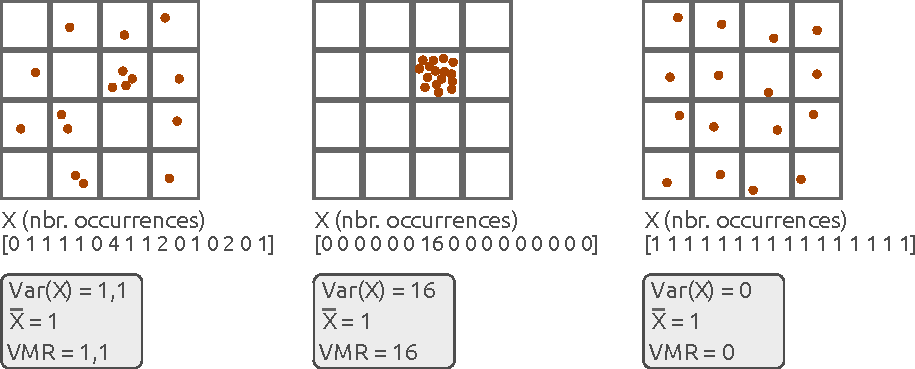
\includegraphics[width=12cm]{VMR.pdf}
\end{figure}

$\rightarrow$ \textbf{test:}  does VMR differs from 1 significantly ? (Student)

\end{frame}


% FRAME
\begin{frame}{Quadrat methods}

« A spatial $\chi^2$»

\begin{itemize}
  \item Construct a regulard grid (quadrats): observed distribution 
  \item Theoretical distribution (null model) is given by a spatial Poisson process.
  \item Contingency tables with  observed and expected occurrences
\end{itemize}

$\rightarrow$ \textbf{test:} Observations differ significantly from expected values ?  ($\chi^2$ test)

\end{frame}

